\chapter{Literature Review}
\label{chap:literature-review}

This chapter will detail the consensus solution for linear elastic stress intensity factors, historical development of failure assessment standards, limits of single-parameter fracture, and estimation techniques for elastic-plastic fracture parameters\footnote{\Cref{chap:app-intro-fracture} provides an overview of the basis of linear elastic fracture mechanics and elastic-plastic fracture mechanics.}.
Finally, this chapter will review ASTM E2899, related tools for analysis of surface cracks in tension, and techniques to ensure accurate and reliable results for analysis of surface cracks in bending.
These are three key components that will be expanded upon in this research.

\section{Consensus Bending Stress Intensity Factor Solution}

A consensus solution for linear elastic stress intensity factors in tension or bending was achieved after many years of discussion and debate.
For example, the Society for Experimental Stress Analysis~\cite{sesa1980} reviewed a range of both numerical and experimental methods for calculating or measuring stress intensity and summarized the relative accuracy and deficiencies in the methods.
Examples of the range of stress intensity solutions are given in \Cref{fig:prior_research_1,fig:prior_research}.
Scott and Thorpe~\cite{scottthorpe1981} reviewed several numerical methods for calculating stress intensity, and identified where the methods diverged substantially.
ASTM E2899 provides a general equation for calculating the linear elastic stress intensity factor \KI for combined tension and bending loading at any position \(\phi\) along the crack front, first published by Newman, Raju, et al. \cite{newmanraju1983a,newmanreuter2000}.
In the absence of applied tension, these equations can be simplified to \Crefrange{eq:e2899-ki}{eq:e2899-g2}.
\begingroup
\allowdisplaybreaks
\begin{align}
\KI &= (
        H \sigma_\text{b} F_\text{b}
        ) \left(\frac{\pi a}{Z}\right)^{0.5} \label{eq:e2899-ki} \\
\sigma_\text{b} &= \frac{6 M}{W t^2} \\
Z &= 1 + 1.464\left(\frac{a}{c}\right)^{1.65} \\
F_\text{b} &= \left[ M_1 + M_2 \left( \frac{a}{t} \right)^2 + M_3 \left( \frac{a}{t} \right)^4 \right] f_\phi f_\text{wb} g \\
M_1 &= 1.13 - 0.09 \left( \frac{a}{c} \right) \\
M_2 &= -0.54 + \left( \frac{0.89}{0.2 + \frac{a}{c}} \right) \\
M_3 &= 0.5 - \frac{1.0}{0.65+\frac{a}{c}} + 14\left( 1.0 - \frac{a}{c} \right)^{24} \\
f_\phi &= \left[ \left( \frac{a}{c} \right)^2 \cos^2 \phi + \sin^2 \phi \right]^{0.25} \\
f_\text{wb} &= \left\{ \sec \left[ \left( \frac{\pi c}{W} \right) \left( \frac{a}{t} \right)^{0.5} \right] \right\}^{0.5} \\
g &= 1+ \left[ 0.1 + 0.35 \left( \frac{a}{t} \right)^2 \right] (1 - \sin \phi)^2 \\
H &= H_1 + (H_2 - H_1) (\sin \phi)^p \\
p &= 0.2 + \frac{a}{c} + 0.6 \left( \frac{a}{t} \right) \\
H_1 &= 1 - 0.34 \left( \frac{a}{t} \right) - 0.11 \frac{a}{c} \left( \frac{a}{t} \right) \\
H_2 &= 1 + G_1 \left( \frac{a}{t} \right) + G_2 \left( \frac{a}{t} \right)^2 \\
G_1 &= -1.22 - 0.12 \left( \frac{a}{c} \right) \\
G_2 &= 0.55 - 1.05 \left( \frac{a}{c} \right)^{0.75} + 0.47 \left( \frac{a}{c} \right)^{1.5} \label{eq:e2899-g2}
\end{align}
\endgroup
These equations are derived from curve fits to finite element results, and popular fracture mechanics software including NASGRO and AFGROW use this consensus solution as the basis for their stress intensity calculations, but no comparable equation exists for the elastic-plastic fracture parameter \J.

\section{Failure Assessment Diagrams and Fitness for Purpose Standards}

Through the 1960s, structural discontinuities including porosity and weld slag inclusion were identified with non-destructive testing (NDT)\nomenclature[1N]{NDT}{Non-destructive testing} and classified by volumetric size \citep{WIESNER2000883}.
These methods could easily overlook planar discontinuities such as cracks, and the repairs required to correct the larger volumetric discontinuities could introduce additional planar discontinuities,
reducing the overall structural quality.
Fitness for purpose (FFP)\nomenclature[1F]{FFP}{fitness for purpose} standards were created to evaluate discontinuities
in terms of their impact on all aspects of structural integrity.
Prominent FFP standards include the R6 standard \citep{r6-1976} and PD~6493 \citep{pd6493-1991} which was later revised as BS~7910 \citep{bs7910-1999}.
Commonly used in FFP standards, the failure assessment diagram (FAD)\nomenclature[1F]{FAD}{failure assessment diagram} is a method of evaluating if a body will be able to withstand certain applied conditions without failing.
It can be considered an extension of simpler evaluation methods such as a factor of safety against yielding, and is similar to a stress-life or strain-life curve when designing for fatigue.

On a simpler factor of safety calculation, the applied conditions determine a stress state and stress magnitude (maximum normal stress, maximum shear stress, von Mises stress, etc.).
If the stress magnitude exceeds a criteria specific to the material (typically a yield stress), the body is considered to have failed and must be redesigned.
On a stress-life evaluation, the applied conditions determine a stress magnitude, and if the number of cycles required at this magnitude exceeds an experimentally-determined material life for this stress level (a point falling outside the region bounded by the stress-life curve), the body is considered to have failed.

\subsection{Failure Assessment Diagrams for Linear Elastic Behavior}

A typical FAD including fracture criteria (\K or \J) will require calculating a stress criterion from the net section stress near a crack, and calculating a fracture criterion from an appropriate stress intensity or strain energy.
A simple FAD for a cracked body made from a brittle material with purely elastic behavior would require net section stress values to remain below the ultimate strength of the material, and \K values at the crack tip to remain below the critical \KIc value associated with brittle failure.
These criteria are assumed to be independent of each other (as \K is proportional to both crack length and applied stress), resulting in a rectangular region on the FAD signifying conditions where the body does not experience failure shown in \Cref{fig:brittle-fad}.
\begin{figure}
\centering
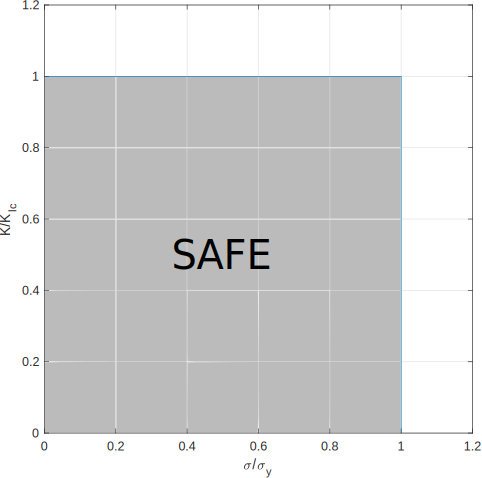
\includegraphics[width=0.6\columnwidth]{brittle-fad-modified}
\caption{\label{fig:brittle-fad} Failure assessment diagram for brittle material}
\end{figure}
Points outside the rectangular region indicate structural failure, either due to fracture or excessive yielding.

\subsection{Failure Assessment Diagrams for Plastic Behavior}

Materials that exhibit some plastic behavior can be stressed beyond their elastic limit, and their locus of failure will be more complicated than a simple rectangle.
A plastic collapse condition, where stress in the body causes plastic hinges to form and the structure becomes geometrically unstable, may be substituted for ultimate strength.
\citet{dowling1975} and Harrison et al. \cite{r6-1976} applied a strip yield model to create one of the first elastic-plastic FADs in the British Central Electricity Generating Board's R6 report.
The effective (plasticity-corrected) stress intensity at the crack tip using a strip yield model is
\begin{align}
\Kef &= \Sy \sqrt{\pi a} \left[ \frac{8}{\pi^2} \ln \sec \frac{\pi \sigma}{2 \Sy} \right]^{\frac{1}{2}}.
\end{align}
The strip yield model is used to account for the effect of the plastic zone on the stress intensity factor \KI.
If the plastic collapse stress \Sc is substituted in place of the yield strength \Sy, this becomes
\begin{align}
\Kef &= \Sc \sqrt{\pi a} \left[ \frac{8}{\pi^2} \ln \sec \frac{\pi \sigma}{2 \Sc} \right]^{\frac{1}{2}}.
\end{align}
Here, the plastic collapse stress is often taken as the average of the material's yield strength \Sy and its ultimate strength \Sut.
If the effective stress intensity is divided by the linear elastic stress intensity factor
\begin{align}
\KI &= \sigma \sqrt{\pi a},
\end{align}
this results in a dimensionless stress intensity ratio
\begin{align}
\frac{\Kef}{\KI} &= \frac{\Sc}{\sigma} \left[ \frac{8}{\pi^2} \ln \sec \frac{\pi \sigma}{2 \Sc} \right]^{\frac{1}{2}}
\end{align}
which can be rewritten in terms of a \K ratio \(\Kr=\frac{\Kef}{\KI}\) and stress ratio \(\Sr = \frac{\sigma}{\Sc} \) as
\begin{align}
\Kr &= \Sr  \left[ \frac{8}{\pi^2} \ln \sec \frac{\pi}{2} \Sr \right]^{\frac{1}{2}},
\end{align}
resulting in a FAD on a normalized scale shown in \Cref{fig:strip-yield-fad}, the R6 curve.
\begin{figure}
\centering
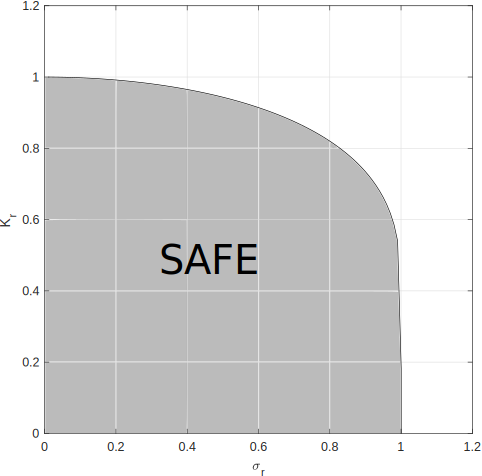
\includegraphics[width=0.6\columnwidth]{strip-yield-fad-modified}
\caption{\label{fig:strip-yield-fad} Failure assessment diagram using strip yield model (R6 curve)}
\end{figure}
Similar to the simpler FAD of \Cref{fig:brittle-fad}, points outside the curve indicate structural failure, whether due mostly to fracture (where \Sr is small, but \Kr is large), mostly to plastic collapse (\(\Sr > 1\)), or a combination of both (e.g., \(\Kr = \Sr = 0.85\)).

If loading paths are added to \Cref{fig:strip-yield-fad}, the resulting graph can show how stable crack growth alters the FFP assessment.
A load path for a stable crack of size \(\frac{a}{W}=0.2\) under monotonically increasing load is shown as the dashed line in \Cref{fig:strip-yield-fad-extra}.
As both \Kr and \Sr are proportional to the applied stress, this is a straight line.
The factor of safety for a load applied to a given crack size is calculated by the ratio of the length of a straight line from the origin to its intersection with the R6 curve versus the length of a straight line segment from the origin to its intersection with a load curve---approximately 2.5 when \(\Sr = 0.25\), or 1.0 when \(\Sr = 0.61\).
\begin{figure}
\centering
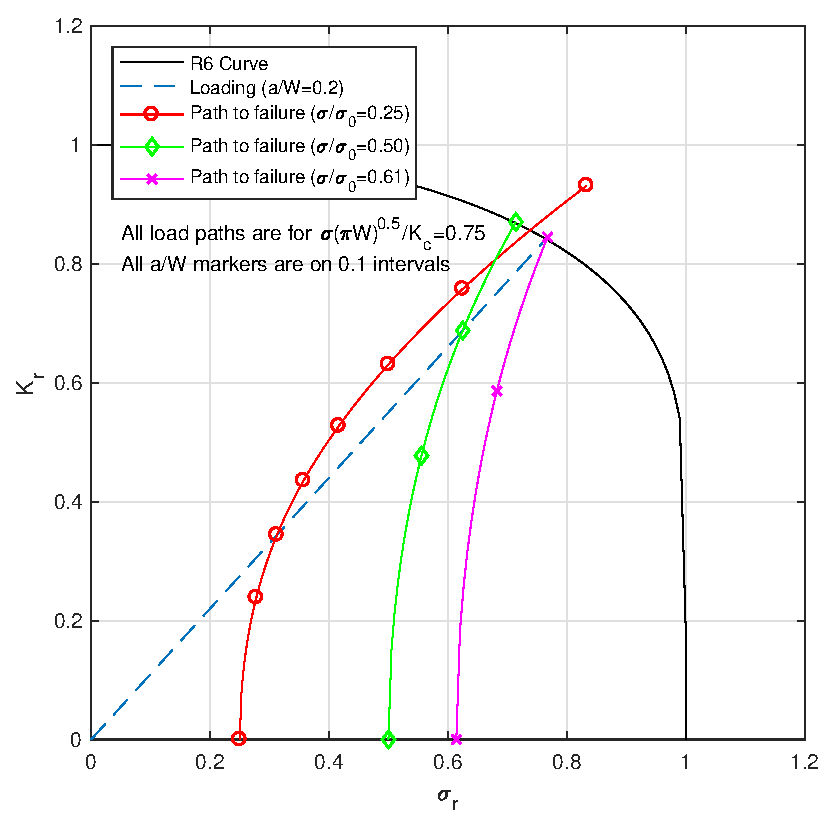
\includegraphics[width=0.6\columnwidth]{strip-yield-fad-extra}
\caption{\label{fig:strip-yield-fad-extra} Failure assessment diagram using strip yield model, including paths to failure}
\end{figure}
\begin{figure}
\centering
\includegraphics[width=0.6\columnwidth]{strip-yield-fad-extra-2}
\caption{\label{fig:strip-yield-fad-extra-2} Failure assessment diagram of material with higher fracture toughness using strip yield model}
\end{figure}
\begin{figure}
\centering
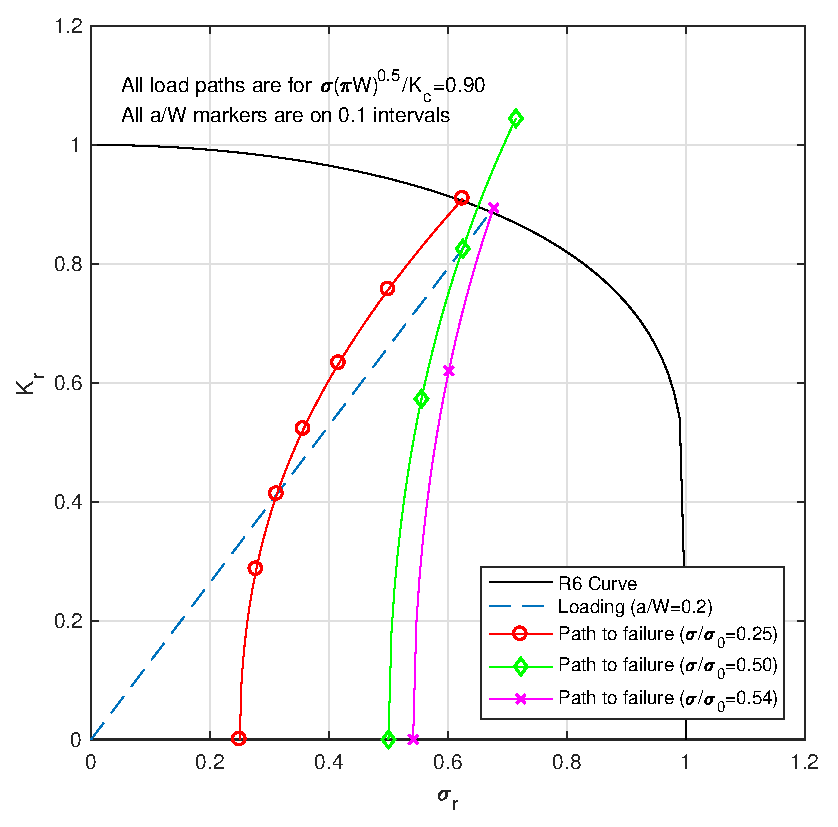
\includegraphics[width=0.6\columnwidth]{strip-yield-fad-extra-3}
\caption{\label{fig:strip-yield-fad-extra-3} Failure assessment diagram of material with lower fracture toughness using strip yield model}
\end{figure}
A material with identical strength but higher fracture toughness is shown in \Cref{fig:strip-yield-fad-extra-2} with the same crack size and initial applied loads.
As expected, the FAD indicates this material is more prone to plastic collapse failure than fracture.
At a given applied load, cracks grow to larger lengths before fracture, and additional load is required to fracture a specimen with a given crack length (\(\frac{\sigma}{\sigma_0} = 0.75\) for \(\frac{a}{W}=0.2\)).
A material with identical strength but lower fracture toughness is shown in \Cref{fig:strip-yield-fad-extra-3} with the same crack size and initial applied loads.
As expected, the FAD indicates this material is more prone to fracture than plastic collapse failure.
At a given applied load, cracks grow to shorter lengths before fracture, and less load is required to fracture a specimen with a given crack length (\(\frac{\sigma}{\sigma_0} = 0.54\) for \(\frac{a}{W}=0.2\)).

\subsection{Failure Assessment Diagrams for Elastic-Plastic Behavior}

Applying a strip-yield model to the failure assessment diagram leads to conservative estimates of failure, since it assumes plastic collapse when net section stresses reach \(\sigma_0\) \citep{kanninen1985}.
For materials that strain harden, the net section becomes stronger and can withstand stresses higher than \(\sigma_0\).
Failure assessment diagrams for elastic-plastic behavior will require both the non-linear stress intensity parameter \J and a strain-hardening material model, such as the Ramberg-Osgood power-law material model given in \Cref{fig:ramberg-osgood}.

The elastic-plastic FAD will depend on material strength, the hardening exponent \(n\), and strain energy in the form of the \J integral. As \J itself depends on specimen geometry and loading configuration, a single FAD curve becomes a family of curves.
\J can be expressed as the sum of an elastic component \Jel and a plastic component \Jpl, with the elastic and plastic components \Jel and \Jpl having the form of
\begin{align}
\Jel(\aapp) &= \tilde{J}_\textnormal{el}(\aapp) \left(\frac{P}{P_0}\right)^2 \\
\Jpl(a, n) &= \tilde{J}_\textnormal{pl}(a, n) \left(\frac{P}{P_0}\right)^{(n+1)}.
\end{align}
At fracture, \(\J = \J_\textnormal{c} = \Jel(\aapp) + \Jpl(a,n)\), and an equivalent to \Kr can be written as

\begin{align}
\J_\textnormal{r} = \frac{\Jel(a)}{\J_\textnormal{c}} &= \frac{\tilde{J}_\textnormal{el}(a) \left(\frac{P}{P_0}\right)^2}{\tilde{J}_\textnormal{el}(\aapp) \left(\frac{P}{P_0}\right)^2 + \tilde{J}_\textnormal{pl}(a, n) \left(\frac{P}{P_0}\right)^{(n+1)}} \nonumber \\
&= \frac{\tilde{J}_\textnormal{el}(a)}{\tilde{J}_\textnormal{el}(\aapp) + \tilde{J}_\textnormal{pl}(a, n) \left(\frac{P}{P_0}\right)^{(n-1)}},
\end{align}
which follows the same trends as \Kr:
as the applied load \(P \rightarrow 0 \),
\( \J_\textnormal{r} \rightarrow \frac{\tilde{J}_\textnormal{el}(a)}{\tilde{J}_\textnormal{el}(\aapp)} = 1 \),
and as \(P \rightarrow \infty \),
\(\tilde{J}_\textnormal{pl} \gg \tilde{J}_\textnormal{el}\), \(\frac{P}{P_0} \rightarrow \infty \) and \(\J_\textnormal{r} \rightarrow 0 \).

The influence of the hardening exponent \(n\) on the FAD for a center-cracked panel in plane stress with \(\frac{a}{W} = 0.5\) is shown in \Cref{fig:fad-ccp-multiple-n} (with \(S_{\text{r}} = \Sr\)), where materials with increased stress hardening are more likely to fail in fracture than in exceeding material strength.
\begin{figure}
\centering
\includegraphics[width=0.7\columnwidth]{FAD-variance-n-modified}
\caption[Failure assessment diagram of center-cracked panel with multiple hardening exponents]{\label{fig:fad-ccp-multiple-n} Failure assessment diagram of center-cracked panel with multiple hardening exponents \cite{epri1981}}
\end{figure}
The influence of plane stress and plane strain conditions on the FAD for a center-cracked panel and a compact tension specimen with \(\frac{a}{W} = 0.5, n = 10\) is shown in \Cref{fig:fad-ccp-ct}.
\begin{figure}
\centering
\includegraphics[width=0.7\columnwidth]{FAD-variance-geometry-modified}
\caption[Failure assessment diagram of center-cracked panel and compact tension specimen]{\label{fig:fad-ccp-ct} Failure assessment diagram of center-cracked panel and compact tension specimen \cite{epri1981}}
\end{figure}
The effect of crack length on a plane strain center-cracked panel with \(n = 10\) is shown in \Cref{fig:fad-crack-lengths}.
\begin{figure}
\centering
\includegraphics[width=0.7\columnwidth]{FAD-variance-aW-modified}
\caption[Failure assessment diagram of center-cracked panel with multiple crack sizes]{\label{fig:fad-crack-lengths} Failure assessment diagram of center-cracked panel with multiple crack sizes \cite{epri1981}}
\end{figure}

\subsection{Failure Assessment Diagrams using Reference Stress Model}

In general, materials can not always be accurately characterized with a power-law curve fit.
But given stress-strain data and the flow stress \(\sigma_0\), \citet{ainsworth1984} defined a reference stress \(\sigma_\textnormal{ref}\) as
\begin{align}
\sigma_\textnormal{ref} &= \frac{P}{P_0}\sigma_0
\end{align}
and a corresponding reference strain \(\epsilon_\textnormal{ref}\) is the total axial strain resulting from applying a uniaxial stress of \(\sigma_\textnormal{ref}\).
Using these values to calculate \Jpl results in
\begin{align}
\Jpl &= \sigma_\textnormal{ref} b \hone \left( \epsilon_\textnormal{ref} - \frac{\sigma_\textnormal{ref} \epsilon_0}{\sigma_0} \right),
\end{align}
where \hone is a dimensionless function of geometry and the power-law exponent \(n\) defined in the EPRI technical report NP-1931 ``Engineering Approach for Elastic-Plastic Fracture Analysis'' \citep{epri1981}.
Though \hone is a function of \(n\), Ainsworth approximated \(\hone(n) \approx \hone(1)\), the \hone value for a linear material.
Though less accurate for low-hardening materials (large values for \(n\)), these materials are already accurately modeled with the simpler strip-yield model.
Ainsworth's approximation for high-hardening materials leads to a simpler \Jpl in terms of the linear elastic stress intensity factor \KI:
\begin{align}
\Jpl &= \frac{\mu \KI^2}{E} \left( \frac{E \epsilon_\textnormal{ref}}{\sigma_\textnormal{ref}} - 1 \right)
\label{eq:jpl-ainsworth}
\end{align}
where \(\mu = 0.75\) for plane strain conditions, and \(\mu = 1.0\) for plane stress conditions.
As \KI values are much more readily found in literature than \hone values, Ainsworth's \Jpl formula can be simpler than EPRI models.

\subsection{Harmonization of Fitness for Purpose Standards}

Each FFP standard attempted to account for multiple modes of structural failure, and experience gained from use of each standard led to the development of encompassing standards with multiple levels of assessment, depending on factors including acceptable levels of conservatism, material type, and available material property data.

While the R6 approach was being developed using strip yield behavior, the British Standards Institute\nomenclature[1B]{BSI}{British Standards Institute} was developing an analogous guide (PD~6493) \cite{pd6493-1991} relating stress to a CTOD-based measurement of fracture toughness and discontinuity size.
Though the initial PD~6493 design curves were conservative in the vast majority of cases, resulting factors of safety ranged from below 1 to over 10 \citep{anderson2005}.
The PD~6493 standard also required separate analysis to determine if the structure was more susceptible to plastic collapse instead of brittle fracture.

A second revision of PD~6493 in 1991 incorporated three levels of assessment, from simplest to most complex.
The Level 1 preliminary assessment added a FAD to the CTOD criteria, so that plastic collapse checks were integrated into the document.
The Level 2 normal assessment was similar to the second edition R6 method, and the Level 3 advanced assessment adapted methods from the third edition R6 standard, including considerations of ductile crack extension \citep{WIESNER2000883}.

In 1999, PD~6493 was converted into a British Standard and designated BS~7910 \cite{bs7910-1999}, and has undergone further revisions and harmonization with other standards including the European FITNET program.
As of 2015 (the latest revision of BS~7910), the ``Level'' terminology was replaced with ``Option'' terminology, and the simplest Level~1 procedure was removed entirely.
Option~1 is conservative, and only requires material data for elastic modulus, yield strength, and ultimate strength.
Option~2 requires a true stress-strain curve, and Option~3 requires use of the \J integral.
Also in the 2015 revision, if crack-tip constraint (the restriction of Poisson effects due to geometry or hydrostatic stress state) can be assessed, it can influence the values used for fracture toughness, and can also affect the equations used to construct the FAD.
These constraint modifications can be applied at any of the three options.
Further background material on constraint and its influence on fracture criteria follows in the next section.

\section{Constraint and Two-Parameter Fracture}

Throughout the preceding section, stress intensity factors, fracture toughness measures, and other quantities have shown a dependency on specimen geometry and plane stress or plane strain conditions, including
plastic zone sizes in \Cref{eq:ry,eq:rp}, \(\frac{a}{W}\) FADs in \Cref{fig:fad-crack-lengths}, and \(\mu\) values in \Cref{eq:jpl-ainsworth}.
These variations are more prominent in the presence of significant plastic deformation, and can be traced back to a general concept of constraint.

Constraint results from conditions that limit or constrain out-of-plane deformation and strain.
Perfectly plane strain conditions are completely constrained in the out-of-plane direction, while perfectly plane stress conditions are completely unconstrained in the out-of-plane direction.
Along the perimeter of a surface crack, the free surface shows little to no constraint, and locations deep within the crack front show higher constraint.

Constraint can also be correlated to the level of stress triaxiality, since large out-of-plane stresses are required to counteract the Poisson's effect that would cause out-of-plane deformation and strain.
Since metals in a plastic state behave similarly to incompressible fluids (\(\nu = 0.5\) instead of \(\nu \approx 0.3\) for an elastic state), this has the effect of limiting the plastic zone size in regions of high constraint.
Higher constraint leads to lower fracture toughness measurements, as a reduced plastic zone size limits ductile behavior of the metal, effectively making it more brittle.

\citet{williams1957} developed an infinite power series form of stress fields near a crack tip of the form
\begin{align}
\sigma_{ij} &= O(r^{-\frac{1}{2}}) + O(r^0) + O(r^{\frac{1}{2}}) + O(r^{\frac{1}{2}}) + \cdots
\end{align}
where the first term is of the form of \Cref{eq:singularity} and dominates the stress values closest to the crack tip.
The third and higher terms in the Williams series vanish near the crack tip, but the second term remains constant, and affects the stress field for values of \(r\) where the magnitude of the singularity term is reduced.

The first two terms of the Williams series for the stress state of a plane strain body subject to Mode I loading are
\begin{align}
\sigma_{ij} &= \frac{\KI}{\sqrt{2\pi r}} f_{ij}(\theta) +
\begin{bmatrix}
T & 0 & 0 \\
0 & 0 & 0 \\
0 & 0 & \nu \T
\end{bmatrix}
\label{eq:t-stress}
\end{align}
where \T is a stress in the \(x\) direction that is a function of the geometry and applied loading, that in turn induces a stress \(\nu \T\) in the \(z\) direction due to plane strain assumptions \citep{anderson2005}.
The single-parameter stress field of \Cref{eq:singularity} where \(\T = 0\) only applies in the limiting case where the plastic zone size is tiny compared to the crack size and the size of the body.

For other cases (\(\T \neq 0\)), \citet{cr5970} performed a modified boundary layer analysis of the region surrounding the crack tip.
Variations in \T affected the \(y\) direction stresses, with \(\T=-\sigma_0 \) values reducing stresses by up to 45\% as shown in \Cref{fig:mbl}.
\begin{figure}
\centering
\includegraphics[width=0.8\columnwidth]{stress-mbl}
\caption[Stress fields from modified boundary layer analysis]{\label{fig:mbl} Stress fields from modified boundary layer analysis \citep{anderson2005}}
\end{figure}
As \T scales with applied stress similarly to \KI, a non-dimensional measure of stress biaxiality \(\Be\) can be defined as
\begin{align}
\Be &= \frac{T \sqrt{\pi a}}{\KI}
\end{align}
and is only a function of cracked body configuration and relative crack size as shown in \Cref{fig:biaxiality}.
\begin{figure}
\centering
\includegraphics[width=0.8\columnwidth]{biaxiality}
\caption[Biaxiality ratio for various cracked body geometries and loading conditions]{\label{fig:biaxiality} Biaxiality ratio for various cracked body geometries and loading conditions \citep{anderson2005}}
\end{figure}

The stress state from \Cref{fig:mbl} could be written as either
\begin{align}
\Sigij &= \left( \Sigij \right)_\textnormal{HRR} + \left( \Sigij \right)_\textnormal{Diff}
\intertext{or}
\Sigij &= \left( \Sigij \right)_{T=0} + \left( \Sigij \right)_\textnormal{Diff} \label{eq:difference-field}
\end{align}
where \(\left( \Sigij \right)_\textnormal{Diff}\) is the difference between \Sigij and the corresponding baseline stress state.
For the second case, using \(\left( \Sigij \right)_{T=0}\) as the baseline, it can be seen that
\(\left( \Sigij \right)_\textnormal{Diff}\)
is relatively constant with respect to distance from the crack tip.
\citeauthor{odowdshih1991} \cite{odowdshih1991, odowdshih1992} extended that approximation to all points forward of the crack tip.
Additionally, they found that
\begin{gather}
\left( \Sxx \right)_\textnormal{Diff} \approx \left( \Syy \right)_\textnormal{Diff}
\gg \left( \sigma_{xy} \right)_\textnormal{Diff}
\end{gather}
indicating that the \T stress effectively causes a hydrostatic shift in stress ahead of the crack tip, dependent on a single parameter \Q.
Thus, \Cref{eq:difference-field} can be rewritten as
\begin{align}
\Sigij &= \left( \Sigij \right)_{T=0} + Q \Szero \deltaij \label{eq:Q-field}
\end{align}
where \deltaij is the Kronecker delta.
\Q has typically been calculated as
\begin{align}
\Q &= \frac{\Syy - \left(\Syy\right)_{T=0}}{\Szero} \text{\quad at } \theta = 0 \text{ and } \frac{r \Szero}{\J} = 2.
\end{align}
\Q and \T have a one-to-one relationship at a given hardening exponent \(n\) as shown in \Cref{fig:q-vs-t}, and \Cref{fig:q-vs-J} shows that \Q remains close to the small-scale yielding value of 0 over a wide range of deformations for bend specimens, versus rapidly dropping with any deformation for center-cracked specimens.

The trend of critical \J values over a range of constraint conditions is shown in \Cref{fig:j-q-experiments}.
Though considerable scatter is present, there is a clear trend that negative \Q values (and correlated negative \T stresses) lead to higher fracture toughness measurements when the failure mechanism is stress-controlled.
As the crack driving force increases, fracture will occur as the \J-\Q curve passes through the shaded region of \Cref{fig:j-q-application}.
\begin{figure}
\centering
\includegraphics[width=0.7\columnwidth]{q-t}
\caption[Relationship between \Q and \T as a function of hardening exponent \(n\)]{\label{fig:q-vs-t} Relationship between \Q and \T as a function of hardening exponent \(n\) \citep{anderson2005}}
\end{figure}
\begin{figure}
\centering
\includegraphics[width=0.7\columnwidth]{q-deflection}
\caption[Relationship between \Q and \J as for two geometries]{\label{fig:q-vs-J} Relationship between \Q and \J as for two geometries \citep{anderson2005}}
\end{figure}
\begin{figure}
\centering
\includegraphics[width=0.7\columnwidth]{j-q-experiments}
\caption[Experimental \J values over a range of \Q values]{\label{fig:j-q-experiments} Experimental \J values over a range of \Q values \citep{anderson2005}}
\end{figure}
\begin{figure}
\centering
\includegraphics[width=0.7\columnwidth]{j-q-application}
\caption[\J-\Q locus]{\label{fig:j-q-application} \J-\Q locus \citep{anderson2005}}
\end{figure}

\FloatBarrier
\section{Methods for Elastic-Plastic and Fully-Plastic Bending Analysis}

This section will detail a selection of methods used to calculate or estimate \J, both numerically and experimentally.
These methods include the adaptation of the contour integral form of \J to a domain integral formulation suitable for finite element analysis, handbook and tabular methods for calculating \J and \K, and the load separation technique for estimating \J from experimental load-displacement records.

\subsection{Numerical Methods}

Though \J is commonly expressed as a contour integral as in \Cref{eq:j-contour-integral}, that formulation does not easily lend itself to numerical evaluation for finite element analysis.
The contour integral form of \J can be rewritten as an equivalent domain integral for a discretized finite element model, as shown in \cite{anderson2005,warp3d,doddsvargas1988}.
For a surface crack model in three dimensions, the domain is a volume of elements surrounding a particular point on the crack front, with a local coordinate system (\(x_1, x_2, x_3\)) with its origin at the crack tip and the \(x_1\) direction oriented toward the direction of crack extension as shown in \Cref{fig:domain-integral-volume}.
\begin{figure}[tbp]
\centering
\includegraphics[width=0.8\textwidth]{domain-integral-volume}
\caption[Example of a domain integral volume for numerically calculating \J]{\label{fig:domain-integral-volume} Example of a domain integral volume for numerically calculating \J \citep{warp3d}}
\end{figure}

For a group of elements centered on the (\(x_1, x_2, x_3\)) origin, \J can be calculated as
\begin{align}
J &= \sum_{\substack{\text{all elements}\\\text{in domain}}} \, \sum_{p=1}^{m} 
  \left\{
    \left[
      \left( 
        \sigma_{ij} \pderiv{u_j}{x_1} - w \delta_{1i}
      \right)
      \pderiv{q}{x_i}
    \right]
    \left|
      \pderiv{x_j}{\xi_k}
    \right|
  \right\}
  w_p
\end{align}
with \(w\) equal to the stress work done to an element,
\begin{align}
w &= w^{(\text{e})} + w^{(\text{p})} \\
  &= \Int{\sigma_{ij}}{\epsilon{_{ij}}^{(\text{e})},0,{\epsilon{_{kl}}^{(\text{e})}}} + \Int{S_{ij}}{\epsilon{_{ij}}^{(\text{p})},0,{\epsilon{_{kl}}^{(\text{p})}}}
\end{align}
and a weight function \(q\) that has a value of 1 at the crack tip and 0 along faces \(A_1\), \(A_2\), and \(A_3\) as shown in \Cref{fig:domain-integral-q}, with partial derivatives defined in terms of element shape functions and parametric coordinates as
\begin{figure}[bp]
\centering
\includegraphics[width=0.8\textwidth]{domain-integral-q}
\caption[\(q\) function for a point along the crack front]{\label{fig:domain-integral-q} \(q\) function for a point along the crack front \citep{warp3d}}
\end{figure}
\begin{align}
\pderiv{q}{x_i} &= \sum_{I=1}^n \sum_{k=1}^{3} \pderiv{N_I}{\xi_k} \pderiv{\xi_k}{x_j} q_I \\
\intertext{where}
m &= \text{number of Gauss points per element} \nonumber \\
w_p &= \text{weight factor at Gauss point } p \nonumber \\
n &= \text{number of nodes per element (in this case, 20)} \nonumber \\
q_I &= \text{nodal value of } q \nonumber \\
N_I &= \text{element shape function} \nonumber \\
\xi_i &= \text{parametric coordinates of element} \nonumber \\
\delta_{ij} &= \text{Kronecker delta} \nonumber \\
S_{ij} &= \text{deviatoric stress tensor.} \nonumber
\end{align}

Though the analytical calculation of \J as a contour integral is path-invariant, the numerical calculation of \J in a finite element model exhibits some path-dependent behavior.
To give the analyst an idea of the accuracy of the calculated \J value, most finite element modeling programs calculate \J using progressively larger volumes of elements seen in \Cref{fig:fem-j-domains}, which should cause \J values to converge to an accurate result.
WARP3D calculates its first domain integral using elements at the crack tip, while Abaqus calculates its first domain integral using the first ring of elements surrounding the crack tip elements.
Both programs calculate additional \J domains by including additional rings of elements surrounding the crack tip, making Abaqus' first \J domain equal to WARP3D's second \J domain.
For the purposes of verification and validation, finite element program developers typically recommend ignoring the first few \J domain values, and using larger domains surrounding the crack tip.
\begin{figure}[tbp]
\centering
\begin{minipage}[b]{0.45\columnwidth}
\setbox1=\hbox{\includegraphics[width=\columnwidth]{contour_integral_regions_abaqus}}
\setbox2=\hbox{\includegraphics[width=\columnwidth]{contour_integral_regions_warp3d}}
\raisebox{0.5\ht1-0.5\ht2}{\includegraphics[width=\columnwidth]{contour_integral_regions_warp3d}}
\subcaption{WARP3D}
\end{minipage}
\begin{minipage}[b]{0.45\columnwidth}
\includegraphics[width=\columnwidth]{contour_integral_regions_abaqus}
\subcaption{Abaqus}
\end{minipage}
\caption{\label{fig:fem-j-domains} Elements used in \J calculations}
\end{figure}

\subsection{Estimation Schemes}
\label{sec:estimation}

Though it is possible to calculate \J using the domain integral method of the previous section, considerable effort would be required to produce finite element models for each geometry and material.
Estimation schemes typically use curve-fitted equations derived from numerical or experimental results, and may include other simplifying assumptions to reduce analytical requirements of calculating \J.

\subsubsection{EPRI Method}
The EPRI technical report ``Engineering Approach for Elastic-Plastic Fracture Analysis'' \citep{epri1981} provided a handbook approach to elastic-plastic fracture mechanics developed for through crack geometries.
The method first assumes that \J is the sum of an elastic component \Jel and a plastic component \Jpl{}.
\begin{align}
\J &= \Jel + \Jpl \label{eq:epri-j}
\end{align}
The elastic component \Jel is defined as in \Cref{eq:j-g}: \(\Jel = \frac{\KI^2}{E'}\).
\KI is calculated using an apparent crack size:
\begin{align}
\aapp &= a_0 + \phi \ry
\intertext{where}
\ry &= \frac{1}{\beta \pi} \left( \frac{n-1}{n+1} \right) \left( \frac{K}{\sigma_0} \right)^2 \\
\beta &=
  \begin{cases}
  2 & \textnormal{for plane stress} \\
  6 & \textnormal{for plane strain}
  \end{cases} \\
\phi &= \frac{1}{1+\left(\frac{P}{P_0}\right)^2} .
\end{align}
The limit load per unit thickness \(P_0\)\nomenclature[1P]{\(P_0\)}{limit load per unit thickness} is calculated from the amount of load required to cause yielding on the net cross section of uncracked material.
For a center-cracked plate loaded in tension:
\begin{align}
P_0 &=
  \begin{cases}
    2 b \sigma_0 & \textnormal{for plane stress} \\
    \frac{4}{\sqrt{3}} b \sigma_0 & \textnormal{for plane strain}
  \end{cases}
\end{align}
where \(b\)\nomenclature[1b]{\(b\)}{uncracked ligament} is the uncracked ligament.
Finally, \Jpl, CMOD, and \(\Delta\) can be calculated as:
\begin{align}
\Jpl &= h_1 \left( \frac{a}{W}, n \right) \left( \frac{P}{P_0} \right)^{n+1} \alpha \epsilon_0 \sigma_0 b \\
\textnormal{CMOD} &= h_2 \left( \frac{a}{W}, n \right) \left( \frac{P}{P_0} \right)^{n} \alpha \epsilon_0 a \\
\Delta &= h_3 \left( \frac{a}{W}, n \right) \left( \frac{P}{P_0} \right)^{n} \alpha \epsilon_0 a \\
\deltat &= \alpha \epsilon_0 b h_4 \left( \frac{a}{W}, n \right) \left( \frac{P}{P_0} \right)^{n+1} \\
       &= d_n \frac{\Jpl}{\sigma_0}
\end{align}
where \hone, \htwo, and \hthree can be found from tables or graphs in \cite{epri1981}.
One such graph is reproduced in \Cref{fig:h1-h2-h3-ccp-plane-strain}.
\hfour is calculated as \(\hfour = d_n \hone\), where \(d_n\) is given in \Cref{fig:dn-plane-strain} for \(\alpha=1\), or
\begin{align}
d_n &= \alpha^{\frac{1}{n}} \left. d_n \right|_{\alpha=1}
\end{align}
for all \(\alpha \neq 1\).
\begin{figure}
\centering
\includegraphics[width=0.8\columnwidth]{h1-h2-h3-ccp-plane-strain}
\caption{\label{fig:h1-h2-h3-ccp-plane-strain} Example EPRI parameters}
\end{figure}
\begin{figure}
\centering
\includegraphics[width=0.8\columnwidth]{dn-plane-strain-modified}
\caption[CTOD parameter for \(\alpha=1\)]{\label{fig:dn-plane-strain} CTOD parameter for \(\alpha=1\) \citep{epri1981}}
\end{figure}

\subsubsection{NASGRO Equation}

The NASGRO suite of fracture mechanics and fatigue crack growth programs \citep{nasgro2000} includes a life assessment program NASFLA for calculating stress intensity factors and crack growth rates for a wide variety of model geometry, material models, and boundary conditions.
Early versions of NASFLA used the Newman-Raju solution for its surface crack growth models.
Later versions include a table of correction factors \(F_\text{p}(\frac{2c}{W}, \frac{a}{c}, \frac{a}{t})\) derived from finite element models for the angles \(\phi = 0\) and \(\phi =\frac{\pi}{2}\).
Selected values of \(F_\text{p}\) are given in \Cref{tab:nasgro-c-tip,tab:nasgro-a-tip}.
The NASGRO stress intensity factor equation is
\begin{align}
\KI &= F_\text{p} \St \sqrt{\frac{\pi a}{Q}} \label{eq:nasgro-ki}
\end{align}
where
\begin{align}
Q &= 1 + 1.464 \left( \frac{a}{c} \right)^{1.65}
\end{align}
is the shape factor of the ellipse representing the crack front.
\begin{table}
\caption[Selected NASGRO stress intensity correction factors $F_\text{p}$ for $\phi=0$]{\label{tab:nasgro-c-tip} Selected NASGRO stress intensity correction factors $F_\text{p}$ for $\phi=0$ \citep{nasgro2000}}
\centering
\begin{tabular}	{ccccccc} \toprule
& & \multicolumn{5}{c}{\(\frac{a}{t}\)} \\ \cmidrule(lr){3-7}
\multicolumn{1}{c}{\(\frac{2c}{W}\)} & \multicolumn{1}{c}{\(\frac{a}{c}\)} & 0.00 & 0.20 & 0.50 & 0.80 & 1.00 \\ \midrule
0.0 & 0.20 & 0.5622 & 0.6110 & 0.7802 & 1.1155 & 1.4436 \\
0.0 & 0.40 & 0.6856 & 0.7817 & 0.9402 & 1.1583 & 1.3383 \\
0.0 & 1.00 & 1.1365 & 1.1595 & 1.2328 & 1.3772 & 1.5145 \\
0.1 & 0.20 & 0.5685 & 0.6133 & 0.7900 & 1.1477 & 1.5014 \\
0.1 & 0.40 & 0.6974 & 0.7824 & 0.9456 & 1.2008 & 1.4256 \\
0.1 & 1.00 & 1.1291 & 1.1544 & 1.2389 & 1.3892 & 1.5273 \\
\vdots & \vdots & \vdots & \vdots & \vdots & \vdots & \vdots \\
1.0 & 1.00 & 1.3956 & 1.8446 & 2.6292 & 3.6964 & 4.5865 \\ \bottomrule
\end{tabular}
\end{table}
\begin{table}
\caption[Selected NASGRO stress intensity correction factors $F_\text{p}$ for $\phi=\frac{\pi}{2}$]{\label{tab:nasgro-a-tip} Selected NASGRO stress intensity correction factors $F_\text{p}$ for $\phi=\frac{\pi}{2}$ \citep{nasgro2000}}
\centering
\begin{tabular}	{ccccccc} \toprule
& & \multicolumn{5}{c}{\(\frac{a}{t}\)} \\ \cmidrule(lr){3-7}
\multicolumn{1}{c}{\(\frac{2c}{W}\)} & \multicolumn{1}{c}{\(\frac{a}{c}\)} & 0.00 & 0.20 & 0.50 & 0.80 & 1.00 \\ \midrule
0.0 & 0.20 & 1.1120 & 1.1445 & 1.4504 & 1.7620 & 1.9729 \\
0.0 & 0.40 & 1.0900 & 1.0945 & 1.2409 & 1.3672 & 1.4404 \\
0.0 & 1.00 & 1.0400 & 1.0400 & 1.0672 & 1.0883 & 1.0800 \\
0.1 & 0.20 & 1.1120 & 1.1452 & 1.4595 & 1.7744 & 1.9847 \\
0.1 & 0.40 & 1.0900 & 1.0950 & 1.2442 & 1.3699 & 1.4409 \\
0.1 & 1.00 & 1.0400 & 1.0260 & 1.0579 & 1.0846 & 1.0820 \\
\vdots & \vdots & \vdots & \vdots & \vdots & \vdots & \vdots \\
1.0 & 1.00 & 1.0400 & 1.2613 & 1.4890 & 1.4558 & 1.3010 \\ \bottomrule
\end{tabular}
\end{table}

\subsection{Load Separation}

\label{sec:intro-load-separation}

\citet{sharobeamlandes1991} reviewed several previous papers as background to their work on calculating \J from a single specimen.
Previously, \J for an edge-cracked plate was defined in terms of an energy rate
\begin{alignat}{2}
\J &=& - \left. \pderiv{U}{A} \right|_{\Delta=\textnormal{constant}} \\
   &=& - \frac{1}{t} \left. \pderiv{U}{a} \right|_{\Delta=\textnormal{constant}}
\end{alignat}
where \(U\) is the strain energy measured as the area under the load-dis\-place\-ment curve, and \(\Delta\)\nomenclature[2\Delta]{\(\Delta\)}{specimen displacement} is a characteristic specimen displacement.
This method required several specimens to determine, since \J was a function of the crack length \(a\).
Recognizing that specimen load was itself a composite function of crack length and material properties, it was reasonable to think that perhaps \J could be separated into geometric and material components.
\citet{riceparismerkle1973} divided \J into elastic and plastic components
\begin{align}
\J &= \Jel + \Jpl .
\end{align}
This form of \J could be rewritten as
\begin{align}
\J &= \etael \frac{A_\textnormal{el}}{b} + \etapl \frac{A_\textnormal{pl}}{b} \label{eq:j-eta}
\end{align}
where
\(A_\textnormal{el}\)\nomenclature[1Ael]{\(A_\textnormal{el}\)}{area under elastic region of load-dis\-place\-ment record} is the area under the elastic region of the load-dis\-place\-ment record, 
\(A_\textnormal{pl}\)\nomenclature[1Apl]{\(A_\textnormal{pl}\)}{area under plastic region of load-dis\-place\-ment record} is the area under the plastic region of the load-dis\-place\-ment record, and both \etael and \etapl are functions of the crack length to specimen width ratio \(\frac{a}{W}\).\nomenclature[2eta]{\(\eta\)}{multiplicative factor for load-dis\-place\-ment record used to calculate \J}
\citet{turner1980} showed that for materials that were not purely elastic or perfectly plastic, a single value of \(\eta\) could be used for the entire specimen record.
Rice estimated \(\eta\) for a center-cracked tension specimen as \(\eta = 1\), and Landes estimated \(\eta = 0.963\) using the load separation method.

If the load can be separated into geometric and material components as
\begin{align}
P &= G \left( \frac{a}{W} \right) H \left( \frac{\Deltapl}{W} \right)
\end{align}	
where \Deltapl \nomenclature[2Deltapl]{\Deltapl}{plastic component of specimen displacement} is the plastic component of a specimen displacement (typically a load-line displacement), then the loads on specimens with different initial crack lengths \(a_i\) and \(a_j\) at a given plastic displacement can be related by a single parameter \(\Sij = \frac{P(a_i)}{P(a_j)}\) as follows:
\begin{align}
\Sij = \left. \frac{P(a_i)}{P(a_j)} \right|_{\Deltapl} &= \left. \frac{P(a_i,\Deltapl)}{P(a_j,\Deltapl)} \right|_{\Deltapl} \\
     &= \frac{G \left( \frac{a_i}{W} \right) H \left( \frac{\Delta_1}{W} \right)}{G \left( \frac{a_i}{W} \right) H \left( \frac{\Delta_1}{W} \right)}
     = \frac{G \left( \frac{a_j}{W} \right) H \left( \frac{\Delta_2}{W} \right)}{G \left( \frac{a_j}{W} \right) H \left( \frac{\Delta_2}{W} \right)} \\
     &= \frac{G \left( \frac{a_i}{W} \right)}{G \left( \frac{a_j}{W} \right)} .
\end{align}
If \Sij\nomenclature[1Sij]{\Sij}{load separation separation parameter} is a constant for the entire range of \Deltapl values examined, then the load \(P\) can be split into separable components. An example of the calculation of \Sij is shown in \Cref{fig:load-separation}.
\begin{figure}
\centering
\includegraphics[width=0.6\columnwidth]{load-sep-final}
\caption[Load separation parameter versus plastic displacement for a compact tension specimen]{\label{fig:load-separation} Load separation parameter versus plastic displacement for a compact tension specimen \citep{sharobeamlandes1991}}
\end{figure}
Previous papers have calculated \etapl from \J as
\begin{align}
\J &= - \left| \pderiv{U}{a} \right|_{\Deltapl} = \etapl \frac{A_\textnormal{pl}}{b} \\
\etapl &= \frac{- \left| \pderiv{U}{a} \right|_{\Deltapl}}{\frac{A_\textnormal{pl}}{b}} .
\end{align}
\citet{sharobeamlandes1991} use the separable form of \(P\) and solve for \etapl as
\begin{align}
\etapl &= \frac{G' \left( \frac{a}{W} \right)}{G \left( \frac{a}{W} \right)} \frac{b}{W} \\
G' \left( \frac{a}{W} \right) &= \D{{G\left(\frac{a}{W}\right)}}{\left(\frac{a}{W}\right)} \\
                              &= - \D{{G\left(\frac{b}{W}\right)}}{\left(\frac{b}{W}\right)}
\end{align}
since \(b=W-a\).

Finally, to find \etapl from \Sij, a log-log plot of \Sij against \(\frac{b_i}{W}\) is linear as shown in \Cref{fig:sij-b-w}, indicating that \Sij has a form
\begin{align}
\Sij &= A_1 \left( \frac{b_i}{W} \right)^m \label{eq:sij-b-w} \\
 A_1 &= \left( \frac{b_j}{W} \right)^{-m} .
\end{align}
Similarly, \Cref{eq:sij-b-w} implies that the geometry function \(G(\frac{b_i}{W})\) follows a power law:
\begin{align}
G\left(\frac{b_i}{W}\right) &= A\left( \frac{b_i}{W} \right)^m
\end{align}
and
\begin{align}
\etapl &= \frac{b_i}{W} \frac{m \left(\frac{b_i}{W}\right)^{m-1}}{\left( \frac{b_i}{W} \right)} = m .
\end{align}
\begin{figure}
\centering
\includegraphics[width=0.55\columnwidth]{load-separation-uncracked-ligament}
\caption[Load separation parameter versus uncracked ligament]{\label{fig:sij-b-w} Load separation parameter versus uncracked ligament \citep{sharobeamlandes1991}}
\end{figure}

Using load separation, \citet{wilsonmani2002} determined \(\etapl\) as a function of the hardening exponent \(n\) as
\begin{align}
\etapl &= 1 - \frac{1}{n}
\intertext{or}
\etapl &= m - \frac{1}{n}
\end{align}
where \(m\) is itself a function of \(n\), and determined that \(m\) varied from 1.022 to 1.069 for plane stress, and from 0.991 to 1.039 for plane strain.

For the surface crack, \citet{sharobeamlandes1994} extended the plastic work factor for through cracks (\etapl) to an equivalent plastic work factor
\begin{align}
\J_{\textnormal{pl,av}} &= \zetapl \int \St d\Delta_{\textnormal{pl,CMOD}} \\
\zetapl &= f\left[ \left( \frac{a}{c}, \frac{a}{t} \right), \textnormal{geometry}, \textnormal{material} \right]
\end{align}
where estimates for \zetapl were found via finite element analysis and load separation. The separation parameter \Sij was written as
\begin{align}
\Sij &= \left[ \frac{\sigma(\frac{a_i}{c_i}, \frac{a_i}{t}, \frac{\Deltapl}{t})}{\St(\frac{a_j}{c_j}, \frac{a_j}{t}, \frac{\Deltapl}{t})} \right]_{\Deltapl}= \frac{G(\frac{a_i}{c_i}, \frac{a_i}{t})}{G(\frac{a_j}{c_j}, \frac{a_j}{t})}
\end{align}
and should be constant for a given material and constraint as shown in \Cref{fig:load-separation-surface-crack}.
\begin{align}
\zetapl &=
  \begin{cases}
  \begin{aligned}
    0.28 +& 0.69 \left( \frac{a}{t} \right) + f_{a,c} + \\
    & \left( 1.835 - 1.67 \left( \frac{a}{t}\right) \right) f_W
  \end{aligned} & 0.1 \leq \frac{a}{t} < 0.5 \\
  0.625 + f_{a,c} + f_W & 0.5 \leq \frac{a}{t} \leq 0.82
\end{cases}
\intertext{where}
f_W &= \frac{t}{W} - 2 \left( \frac{t}{W} \right)^2 \quad (\frac{t}{W}) \leq 0.25, \quad (\frac{c}{W}) \leq 0.25 \\
f_{a,c} &=
  \begin{cases}
  0.22 \left( \sqrt{\frac{a}{t}} - 0.3 \right) \left( \frac{c}{a} -1 \right), & 0.42 \leq \frac{a}{c} \leq 1.0, \frac{a}{t} < 0.5 \\
  0.09 \left( \frac{c}{a} -1 \right), & 0.42 \leq \frac{a}{c} \leq 1.0, \frac{a}{t} \geq 0.5 \\
  -0.08 \left( \frac{a}{c} - 1 \right), & 1.0 \leq \frac{a}{c} \leq 2.0
  \end{cases}
\end{align}
A single-specimen key curve can be constructed by curve-fitting \Sij versus \(\frac{b_e}{t}\), the effective uncracked ligament length from the R6 standard, as shown in \Cref{fig:bet_Sij_original}.
The relationship between the plastic component of CMOD and load line displacement is shown in \Cref{fig:load-separation-cmod-lld-surface-crack}.
Since the two values have a constant ratio over a wide range of \Deltapl values, the equation for \Jpl can be expressed in terms of either measurement.
\begin{figure}
\centering
\includegraphics[width=0.6\columnwidth]{load-separation-surface-crack}
\caption[Separation parameter values for surface cracks at various normalized plastic displacements]{\label{fig:load-separation-surface-crack} Separation parameter values for surface cracks at various normalized plastic displacements \cite{sharobeamlandes1994}}
\end{figure}
\begin{figure}
\centering
\includegraphics[width=0.6\columnwidth]{bet_Sij_original}
\caption[Separation parameter values versus effective uncracked ligament length]{\label{fig:bet_Sij_original} Separation parameter values versus effective uncracked ligament length \cite{sharobeamlandes1994}}
\end{figure}
\begin{figure}
\centering
\includegraphics[width=0.6\columnwidth]{load-separation-cmod-lld-surface-crack}
\caption[Relationship between plastic components of CMOD and load line displacement]{\label{fig:load-separation-cmod-lld-surface-crack} Relationship between plastic components of CMOD and load line displacement \cite{sharobeamlandes1994}}
\end{figure}

\FloatBarrier

\section{Engineering Approaches for Elastic-Plastic and Fully-Plastic Analysis of Surface-Cracked Plates in Bending}

This section will give an overview of ASTM E2899, methods for satisfying its analysis requirements to ensure the validity of experiments, and the limitations of the TASC software tool often used for that analysis.

\subsection{ASTM E2899}

In ASTM E2899 \cite{astme2899}, a semi-elliptical surface starter crack is machined into a flat rectangular plate, and the starter crack is fatigued to induce a sharper crack front.
After the initial fatigue cycles have completed, the plate is subjected to monotonically increasing bending or tension force while the CMOD is monitored.
As the force is applied, either the specimen will fail due to unstable crack growth, or else the initiation of stable crack tearing is detected via methods including electric potential drop, measurement of CMOD, monitoring acoustic emissions, or crack shape replicates.
Once crack growth has been detected, the angular position where crack growth occurs (\(\phi_i\)) is recorded, and material properties and crack-front conditions are used to identify which of the linear elastic, elastic-plastic, or fully-plastic (field collapse) regimes are applicable to the specimen and loading condition.
If either the linear elastic or elastic-plastic regimes are applicable, constraint measures at \(\phi_i\) are calculated from tables, and if the constraint value is negative, both the constraint and the value of \K at \(\phi_i\) (for linear elastic) or \J at \(\phi_i\) (for elastic-plastic) is reported.
If the constraint value is positive, only \K or \J is reported.
For the linear elastic regime, Annex A1 of ASTM E2899 provides a series of 19 equations that provide accurate estimations of \KI for \(\frac{a}{c} \leq 1\) and \(\frac{a}{t} \leq 0.8\).
No such set of equations exists for the elastic-plastic regime, thus other methods must be employed to calculate \J.
Annex A6 of ASTM E2899-15 recommends finite element analysis using domain integrals to calculate \J.

The analysis requirements of ASTM E2899 go far beyond earlier standards for measuring fracture toughness.
As seen in \Cref{tab:astm-analysis-requirements},
\begin{table}[tbp]
\caption{\label{tab:astm-analysis-requirements} Analysis Requirements in Several ASTM Standards}
\begin{tabular}{c p{0.5\textwidth} p{0.3\textwidth}} \toprule
 & Requirements & Tools \\ \midrule
E8 & Fit linear region of stress-strain curve, offset to find yield strength & Strip chart and calculator \\
E399 & Fit linear region of force-CMOD curve, draw secant line with 5\% less slope, calculate \K with algebraic equations & Strip chart and calculator or spreadsheet \\ 
E740 & Calculate \K with algebraic equations at two positions, report higher value & Calculator or spreadsheet \\
E1820 & Calculate \K with algebraic equations. EPRI method with \Jel calculated from \K and \Jpl calculated from area under load-displacement curve and algebraic equations & Spreadsheet \\ \bottomrule
\end{tabular}
\end{table}
earlier standards can be completed with pocket calculators or simple spreadsheets, tools that are well within reach of any engineer or test facility, and the calculations are easily verified and checked by others.
Only ASTM E2899 requires an elastic-plastic finite element analysis to calculate \J.
Not only is the software used to perform this analysis much more expensive than a spreadsheet or calculator, it requires a much higher level of skill to create an accurate analysis, and is much more difficult for others to verify and check the results.

\subsection{Interpolation}

Performing a finite element analysis for every crack geometry and set of material properties would prove to be quite time-intensive.
It is reasonable to assume that the variation in experimental results from theoretically identical specimens is large enough to allow interpolated results derived from similar geometry and material properties to fall within the range of experimental error.
In that case, the need to perform finite element analysis on every model can be replaced by performing finite element analysis on enough models spanning a range of typical crack geometries and material properties.

\subsection{Tool for Analysis of Surface Cracks (TASC)}

NASA Marshall Space Flight Center (MSFC) has developed a MATLAB program, Tool for Analysis of Surface Cracks (TASC) \citep{allenwells2014, tasc}, to interpolate \J values and surface crack nucleation conditions for a wide range of crack geometries and materials loaded purely in tension.
The development of TASC required the solution of 600 finite element models for geometries spanning
 (\(0.2 \leq \frac{a}{c} \leq 1.0,\; 0.2 \leq \frac{a}{t} \leq 0.8\)) and materials spanning (\(100 \leq \frac{E}{S_{\text{ys}}} \leq 1000,\; 3 \leq n \leq 20\)) shown in \Cref{fig:tasc-geometries,fig:tasc-materials}.
\begin{figure}
\centering
\includegraphics[width=\textwidth]{tasc-geometries}
\caption[Crack geometries used in TASC]{\label{fig:tasc-geometries} Crack geometries used in TASC \citep{allenwells2014}}
\end{figure}
\begin{figure}
\centering
\includegraphics[width=\textwidth]{tasc-materials}
\caption[Material models used in TASC]{\label{fig:tasc-materials} Material models used in TASC \citep{allenwells2014}}
\end{figure}
Results for each model were condensed to a normalized \J as a function of a normalized CMOD and \(\phi\), and the normalized CMOD in terms of a normalized far-field stress as shown in \Cref{fig:tasc-sample-result}.
\begin{figure}
\centering
\includegraphics[width=\textwidth]{tasc-sample-result}
\caption[Sample result used by TASC for interpolations]{\label{fig:tasc-sample-result} Sample result used by TASC for interpolations \citep{allenwells2014}}
\end{figure}
TASC uses normalized geometries and material properties, interpolates intermediate results for any geometry and material property spanned by its database, and then scales the interpolated results back to the true physical parameters of an experiment or model.
As TASC does not currently include support for bending loads, MSFC has expressed interest in extending the TASC code and results database to include bending.
Bending conditions introduce additional complexity to the boundary conditions and crack tip constraint, and will need some additional steps taken to ensure accurate results.
These steps are outlined in the next section.
\FloatBarrier
\section{Verification and Validation}
It is apparent throughout the preceding sections that both analytical and experimental techniques for predicting conditions at a crack front include inherent uncertainty.
Even worse, applying the wrong techniques (for example, using an elastic material model when significant plastic deformation is present) can lead to outright errors.
Deviations between predicted behavior and measured behavior can be attributed to two main causes:
repeatability and accuracy of measurements or calculations,
and
application of the correct models or experimental procedures to include all significant physical effects.
Addressing and correcting issues with repeatability and accuracy is improving verification,
and
addressing and correcting issues with application of models or procedures to include all significant effects is improving validation.%

The U.S. Department of Defense Standard MIL-STD-3022 ``Documentation of Verification, Validation, and Accreditation (VV\&A) for Models and Simulations'' (\citeyear{mil-std-3022}) defines validation as ``the process of determining the degree to which a model, simulation, \ldots{} and their associated data are accurate representations of the real world'', and verification as ``the process of determining that a model, simulation, \ldots{} and their associated data accurately represents the developer's conceptual description and specifications''.
In the domain of software engineering, \citet{boehm1989} summarized validation as part of ``building the right product'' and verification as part of ``building the product right''.

The American Society of Mechanical Engineers ``Guide for Verification and Validation in Computational Solid Mechanics'' (\citeyear{asme-vv}) defines the goal of V\&V as validating a model for its intended use.
In this application, demonstrations of both the model's predictive capability and accuracy are required.
Defining the model's intended use also imposes a set of limitations on the applicability of the model.
An example given is predicting the response of a specific make and model of vehicle to frontal impacts against a rigid wall.
Validation requirements may include predicting the compaction of the front end of the vehicle within 20\% accuracy versus experiments run at 10, 20, and 30~mph.
If a model passes the validation tests, it can be assumed to be useful in predicting compaction at any speed up to 30~mph, but this does not ensure any accuracy for crashes at higher speeds, in different directions, on different frames, or against items other than rigid walls.

Real-world physical systems are often composed of several assemblies.
Each assembly includes multiple subassemblies, and each subassembly is a collection of individual components.
Similarly, a system-level model can be constructed from several assembly models, each of which includes subassembly and component models.
Inaccuracies in lower-level models are typically compounded in higher-level models, which means that a given level of accuracy at the system level requires higher accuracy for subassembly and component models.
For example, a model that calculates the buckling strength of a tubular steel strut to 10\% accuracy may mean the accuracy of a model that calculates the collapse strength of a frame made from the struts to 20\% accuracy.

It should be noted that practical computational limits require simplification of lower-level models when higher-level models are created.
Modeling every component of a complex system to maximum accuracy would make a system-level model that would take a huge amount of time and resources to solve.
For example, a finite element model of a tubular steel strut may use two-dimensional shell elements or three-dimensional solid elements, but the response of the strut can be simplified to a model using one-dimensional (possibly nonlinear) beam elements.
Additional error in higher-level models is due to these simplifications, and also to interaction between components that may be difficult to predict in advance.

\subsection{Model Development}

In ASME V\&V procedures, model development is composed of four tasks:
\begin{enumerate}
\item formulation of conceptual models,
\item converting the conceptual model to a computational model,
\item revising models during V\&V,
and 
\item quantifying sensitivity and uncertainty of parameters in the model.
\end{enumerate}
Model development assumes that the physical system of interest, use of the model, and accuracy requirements have been previously defined.

Development of the conceptual model includes defining fundamental assumptions such as
how many components will be included in the model (fasteners, electronics),
models of material behavior (elastic, elastic-plastic, temperature dependent),
elimination of unimportant geometric features (external rounds, small holes in areas of low stress),
and
selection of boundary conditions (fixed, pinned, free) and component interfaces (bonded, frictionless, frictional).
Inadvertent elimination of important mechanical phenomena may lead to inadequate simulations, while focusing on essential physical processes ensures the model solves quickly and accurately.
Development of conceptual models requires defining response features of interest: the characteristics of the physical system that need to be accurately predicted for the model's intended use.
Constructing a Phenomena Identification and Ranking Table (PIRT) is a common tool in identifying key physical characteristics required for accurate simulation.
The PIRT is normally constructed by a group of subject experts who rank physical processes according to their influence on the response characteristics.
An example of a PIRT is given in \Cref{tab:pirt}.
An additional use of the PIRT is in ranking which phenomena require additional scrutiny during the validation phase: in the example PIRT, validating plasticity may be less important if prior experience indicates that it can be modeled with high confidence.
Fracture may be less important to validate if it has little influence on the response of interest.
On the other hand, interface and loads have a greater influence and less confidence, and would be the focus of validation activities.
\begin{table}[bp]
\caption[PIRT example]{\label{tab:pirt} PIRT example \citep{asme-vv}}
\centering
\begin{tabular}{cccc} \toprule
           &            & Importance to & Level of \\
           & Type of    & Response of   & Confidence \\
Phenomenon & Phenomenon & Interest      & in Model \\ \midrule

A & Interface & High & Medium \\
B & Plasticity & Medium & High \\
C & Loads & Medium & Low \\
D & Fracture & Low & Low \\ \bottomrule
\end{tabular}
\end{table}

Development of computational models starts with converting the assumptions and phenomena in the conceptual model into equations and other mathematical statements.
Specification of the mathematical model also helps define responses in terms of model input parameters, such as loads, material properties, and coefficients of friction.
Once the mathematical model has been defined, it can be converted into a computational model.
The computational model is a numerical implementation that approximates the mathematical model, and can include procedures for spatial and temporal discretization, solution of systems of governing equations, and convergence criteria for iterative solution methods.
The computational model can use an existing simulation code, or one written specifically for the current model.
The model can be as simple or complex as necessary.
The analyst responsible for the computational model must understand the assumptions made during the earlier stages, and the influence of parameters and boundary conditions on the model's results: for example, the influence of end conditions on a buckling problem.

There are two primary causes for model revision: to meet accuracy requirements, or to meet previously-unknown requirements.
There are two general methods for revising the model: adjustment of model parameters, or modifying the form of the model and governing equations.
Updates to model parameters are a method to adjust for common sources of modeling difficulty, such as compliance in joints, energy loss or damping, and uncertainty in boundary conditions.
Parameters are adjusted to bring the model responses closer to experimental values.
However, adjustment of parameters to exactly fit one experiment may inadvertently create worse fits with future experiments.
If parameters can be measured independently, those measurements should drive parameter adjustment.
Modifying the form of the model requires changing the mathematical model (and thus, the computational model).
It is most commonly performed when reasonable experimental uncertainty in parameters cannot account for differences in responses, or when observations of physical behavior in an experiment do not match model assumptions (for example, if assumed planar motion has a significant out-of-plane component, if supports assumed to be rigid show significant compliance, if surfaces assumed to be in constant contact separate from each other, etc.).

Performing a sensitivity analysis of the computational model can highlight previously-unknown phenomena: for example, does reducing the wall thickness slightly cause buckling effects to appear?
It can also point out the relative significance of various model parameters.
Information gathered in the sensitivity study can modify the PIRT, increasing or decreasing the importance of parameters.
Sensitivity analysis should be performed after each model revision, since small changes in the model can cause major changes in responses.

Though uncertainty is obviously a part of an experimental program, it is also present in simulations.
Uncertainties at any stage of development can be broadly classified as aleatory (or irreducible) and epistemic (or reducible).
Aleatory uncertainties are inherent in physical systems, and have root causes in the variation of physical properties and processes.
No manufactured component is free from geometric deviations, no material property has exact textbook values in every specimen, and no assembly is constructed with exact fastener preloading, alignment, etc.
Though this uncertainty can never be eliminated, it can be quantified by conducting tests to establish statistical characteristics for each parameter (mean, variance, distribution type).
Once the uncertainty in parameters is quantified, their variability can be propagated through simulations with probabilistic analysis, setting lower bounds on how much variability will be present in the simulation results.

Epistemic uncertainties are the result of incomplete information or knowledge.
Two major categories of reducible uncertainties are statistical uncertainty and modeling uncertainty.
Statistical uncertainty occurs whenever a limited number of samples is used to establish statistical material properties: if only two or three tests are performed, estimates on the population mean and variance will be much worse than if 30 tests are performed.
Modeling uncertainty can be difficult to quantify, but it derives from assumptions made during modeling.
If a material property is assumed to be constant for the simulation, but in reality is time-dependent, temperature-dependent or otherwise variable, the assumption of constant properties is a source of reducible uncertainty.

\subsection{Verification}

Verification is the process of comparing the computational model to the original mathematical model.
It precedes validation, and examines the computational model in the contexts of numerical analysis, software quality engineering, identification of programming errors, and numerical error estimation.
Verification is divided into two main task areas: code verification and calculation verification.

Code verification is composed of two groups: numerical code verification and software quality engineering (SQE).
Numerical code verification verifies that the solution algorithms are correctly programmed.
This often involves convergence testing with different discretization levels and comparison to known analytical solutions.
Software quality engineering procedures seek to eliminate flaws in both the solution code, and in any underlying libraries, compilers, processors, or other tools used in the calculation.

Calculation verification often builds on convergence studies from the code verification stage, and uses numerical solutions from two different models to determine the influence of mesh size and mesh bias.
Methods normally use either gradient tests or analysis of residuals as either the mesh size or the order of the finite elements change.
One area where calculation verification has problems is around discontinuities or singularities (such as the stress field at a crack tip).

\subsection{Validation}

The goal of validation activities is to assess the model's predictive capability by comparing numerical results to corresponding experimental results.
Proper comparison of results can only occur after the following criteria are satisfied:
\begin{itemize}
\item defining the model's intended use,
\item conclusion of code verification and calculation verification, and
\item quantifying uncertainties in both the numerical and experimental results.
\end{itemize}
The validation experiments must be distinct from any earlier experiments used in the verification stage.
The goal is to design and conduct a set of experiments providing a stringent enough test of the model to establish its predictive capability.
If the model predicts the results of all the validation experiments to the predefined level of accuracy, it is assumed to be validated for its intended use.

\subsection{V\&V Efforts within the Fracture Mechanics Community}

V\&V has been applied in the study of fracture mechanics and fatigue life prediction.
\citet{favanesi1994} performed V\&V activities on the NASCRAC fracture mechanics software, verifying it against the FLAGRO and FRANC2D codes, and also validating it against \citet{tadaparisirwin1973} or their own experimental tests.
The most basic predictions (\K versus \(a\), \J versus \(a\)) were generally verified and validated, but other predictions (proof tests, creep, crack retardation) were either invalid, or the uncertainty in experimental measurements was high enough to make results inconclusive.
\citet{wilson1995} identified problems with both NASCRAC and FLAGRO.
NASCRAC contained two types of errors in its material database: both were related to assuming that certain fracture properties (\Kc and \(m\)) were constant instead of functions of geometry and load.
NASCRAC also showed significant deviations from previously-established fatigue crack growth curves, well beyond the limits of uncertainty, as shown in \Cref{fig:nascrac-vv-tension}.
\begin{figure}
\centering
\includegraphics[width=0.5\columnwidth]{nascrac-vv-tension}
\caption[Comparison between NASCRAC fatigue crack growth curves and previous results]{\label{fig:nascrac-vv-tension} Comparison between NASCRAC fatigue crack growth curves and previous results \citep{wilson1995}}
\end{figure}
The FLAGRO source code, written in FORTRAN, contained several instances of non-portable statements, non-standard use of \verb|COMMON| blocks, and little use of program flow control (\verb|IF/THEN/ELSE| statements).
\citet{mcclung2012} outlines the V\&V process in great detail, and shows an example of verifying a \K solution by comparing the FADD3D, FEACrack, and FLAGRO solvers.
All three were in good agreement through most of the crack front, but FEACrack deviated from the others at \(\phi=0\) and \(\phi=\pi\).
McClung also showed the large amounts of work remaining to complete the V\&V process on fracture mechanics.

The next chapter will build on existing techniques from this chapter, including EPRI estimation, load separation, models used for the TASC database, interpolation, and V\&V to verify results from the literature.
The verification work done will be used to improve the quality of the work required for the current research. 
